\documentclass{rapportCS}
\usepackage{hyperref}
\usepackage{tabularx}
\usepackage{booktabs}
\usepackage{amsmath}
\usepackage{amssymb}
\usepackage{float}

\title{Advanced Spectral Analysis -- Labwork Report}

\begin{document}

%----------- Informations du rapport ---------

\titre{Advanced Spectral Analysis}
\mention{Signal Processing 2}
\trigrammemention{Signal Processing 2}
\master{Deuxième année}
\filiere{Spécialité Physique}

\eleve{Leelou RUSCH}

\dates{2026}

\tuteurecole{~}

\tuteurentreprise{
    \textsc{Stéphane ROSSIGNOL} \\
    stephane.rossignol@centralesupelec.com 
}

%----------- Initialisation -------------------

\fairemarges
\fairepagedegarde

%----------- Abstract -------------------
\vspace*{\stretch{1}}
\begin{center}
	\begin{abstract}
        This report presents the experimental results and theoretical analysis for the four modules of the Advanced Spectral Analysis labwork:
        \begin{enumerate}
            \item \textbf{Fundamental Frequency Estimation ($f_0$):} Comparative study of non-parametric (Short-Time FFT, Autocorrelation) and parametric/subspace methods (Levinson-Durbin LPC, Burg, MUSIC) on speech and instrument signals, including energy-based silence detection, note segmentation, tempo, and vibrato tracking.
            \item \textbf{Filter Banks \& Subband Decomposition:} Two-layer dyadic filter bank tree decomposing a 4-component harmonic signal ($f_0=880$\,Hz, $F_s=8000$\,Hz) into single-tone subbands, with spectral transposition derivations, Hilbert analytic frequency retrieval, and modulated vibrato analysis.
            \item \textbf{Wavelet Denoising \& Source Separation:} Multiresolution Discrete Wavelet Transform (DWT) thresholding (soft/hard operators, Donoho's universal threshold, Monte Carlo SNR optimization) achieving $+9.7$\,dB SNR improvement, and underdetermined source separation ($100$\,Hz and $500$\,Hz) via subband energy masking.
            \item \textbf{Sparse Signal Compression (Pursuit Algorithms):} Audio frame compression over an overcomplete multiscale dictionary ($5.3\times$ redundancy). Performance benchmark of Matching Pursuit (MP), Orthogonal Matching Pursuit (OMP), and Basis Pursuit (BP via FISTA) across SNR, runtime, and compression ratio ($N/K$), alongside runtime comparisons of OMP solvers (Standard LS, QR, Cholesky).
        \end{enumerate}
    \end{abstract}
\end{center}
\vspace*{\stretch{1}}
\newpage

%------------ Table des matières ----------------

\tabledematieres
\newpage

%------------ Corps du rapport ----------------

\section{Detection of Fundamental Frequency ($f_0$)}

\subsection{Context and Audio Characteristics}

The objective of this part is to estimate the fundamental frequency $f_0(t)$ across successive time frames for two monophonic recordings: a sung voice (\texttt{voiceP.wav}, $F_s = 22050$\,Hz, duration $25.57$\,s) and a flute melody (\texttt{fluteircam.wav}, $F_s = 32000$\,Hz, duration $13.69$\,s). Ground truth segmentations (\texttt{veriteterrainvoiceP.txt} and \texttt{veriteterrainflute.txt}) are available to benchmark performance.

Both signals feature rich harmonic content and natural dynamic variations. Acoustic instruments and human phonation also exhibit silence intervals at the beginning, between notes, and at the end of phrases, necessitating robust silence gating before frequency evaluation.

\subsection{Frame Duration and Silence Detection}

\paragraph{Choice of Frame Duration $T_f$:}
To obtain a reliable estimate of the fundamental frequency, each analysis frame must contain at least three complete periods of the lowest expected frequency:
\begin{equation}
    T_f \ge \frac{3}{\min(f_0)}
\end{equation}
For male and female speech as well as flute, fundamental frequencies typically span from $100$\,Hz to $700$\,Hz. With $\min(f_0) \approx 100$\,Hz, we select $T_f = 30$\,ms ($N_f = 960$ samples at $32$\,kHz, and $N_f = 661$ samples at $22.05$\,kHz). This duration guarantees adequate frequency resolution while preserving quasi-stationarity.

\paragraph{Silence Detection via RMS Energy:}
Silence segments consist of low-amplitude background noise. The Root Mean Square (RMS) energy over a frame $x[n]$ of length $N$ is computed as:
\begin{equation}
    \text{RMS} = \sqrt{\frac{1}{N} \sum_{n=0}^{N-1} x[n]^2}
\end{equation}
Frames satisfying $\text{RMS} < \theta_{\text{energy}}$ (with $\theta_{\text{energy}} \approx 0.01$) are labeled as unvoiced/silence ($f_0 = \text{NaN}$), avoiding spurious peak detections in silent regions.

\begin{figure}[H]
    \centering
    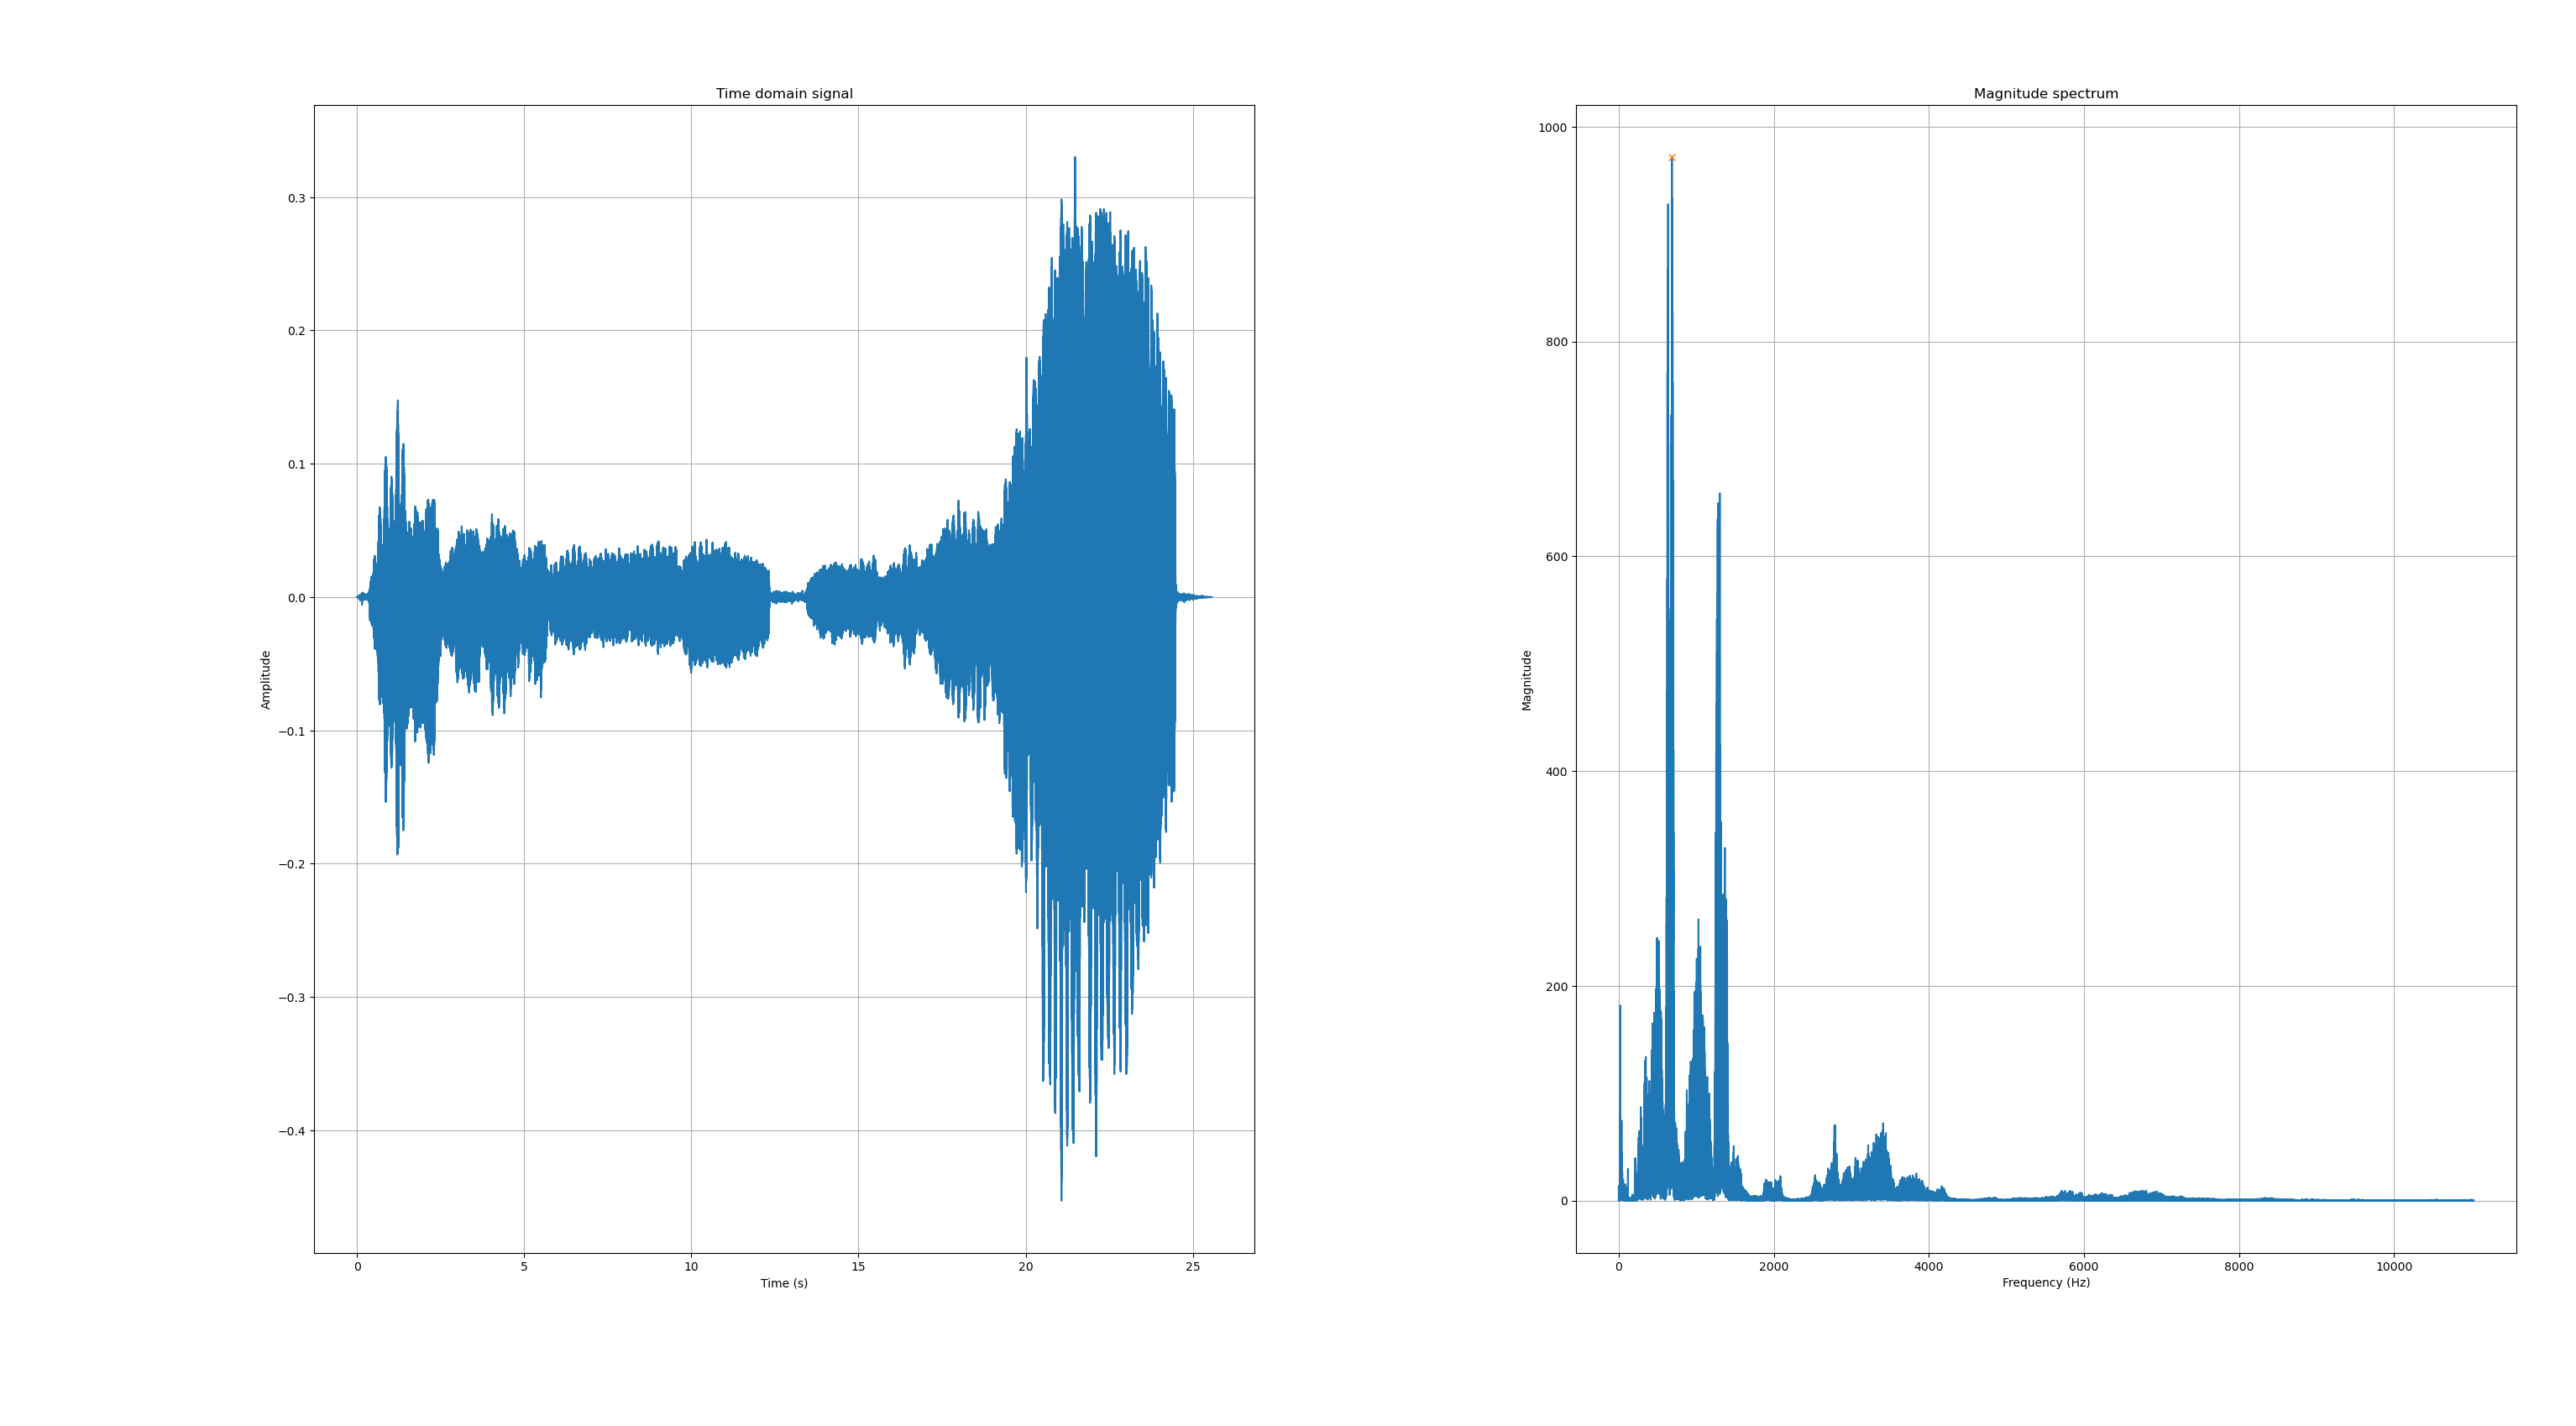
\includegraphics[width=0.82\textwidth]{./images/voiceP_fft_w_f0.png}
    \caption{Frame-by-frame FFT spectrum and estimated fundamental frequency $f_0$ on \texttt{voiceP.wav}.}
    \label{fig:voice_fft}
\end{figure}

\subsection{Pitch Estimation Algorithms}

\subsubsection{Short-Time Fast Fourier Transform (FFT)}
Each frame is windowed by a Hanning window $w[n]$ to minimize spectral leakage, and the discrete spectrum is evaluated via \texttt{scipy.fft.rfft}:
\begin{equation}
    X[k] = \sum_{n=0}^{N-1} x[n] w[n] e^{-j 2\pi k n / N}, \quad k = 0, \dots, N/2
\end{equation}
The pitch is estimated from the frequency corresponding to the maximum magnitude peak:
\begin{equation}
    k_{\max} = \arg\max_k |X[k]| \implies f_{0,\text{FFT}} = \frac{k_{\max} F_s}{N}
\end{equation}
\textbf{Limitation:} When the fundamental frequency contains less energy than higher harmonics (formants in singing voice), $\arg\max$ selects a harmonic ($2f_0$ or $3f_0$) instead of $f_0$, causing pitch halving or octave jumps.

\subsubsection{Autocorrelation Method}
The biased autocorrelation function of the windowed frame $x_w[n]$ is defined for non-negative lags $m \ge 0$ by:
\begin{equation}
    R_{xx}[m] = \frac{1}{N} \sum_{n=0}^{N-1-m} x_w[n] x_w[n+m]
\end{equation}
For periodic signals of period $T_0$, $R_{xx}[m]$ displays local peaks at multiples of the pitch lag $m_0 = T_0 F_s$. By searching for the highest peak in the plausible pitch lag interval $[m_{\min}, m_{\max}]$ corresponding to $f_0 \in [80, 800]$\,Hz:
\begin{equation}
    m_0 = \arg\max_{m \in [m_{\min}, m_{\max}]} R_{xx}[m] \implies f_{0,\text{autocorr}} = \frac{F_s}{m_0}
\end{equation}
Autocorrelation measures the repetition rate of the waveform envelope. It is inherently resilient to missing fundamentals and formant amplification.

\begin{figure}[H]
    \centering
    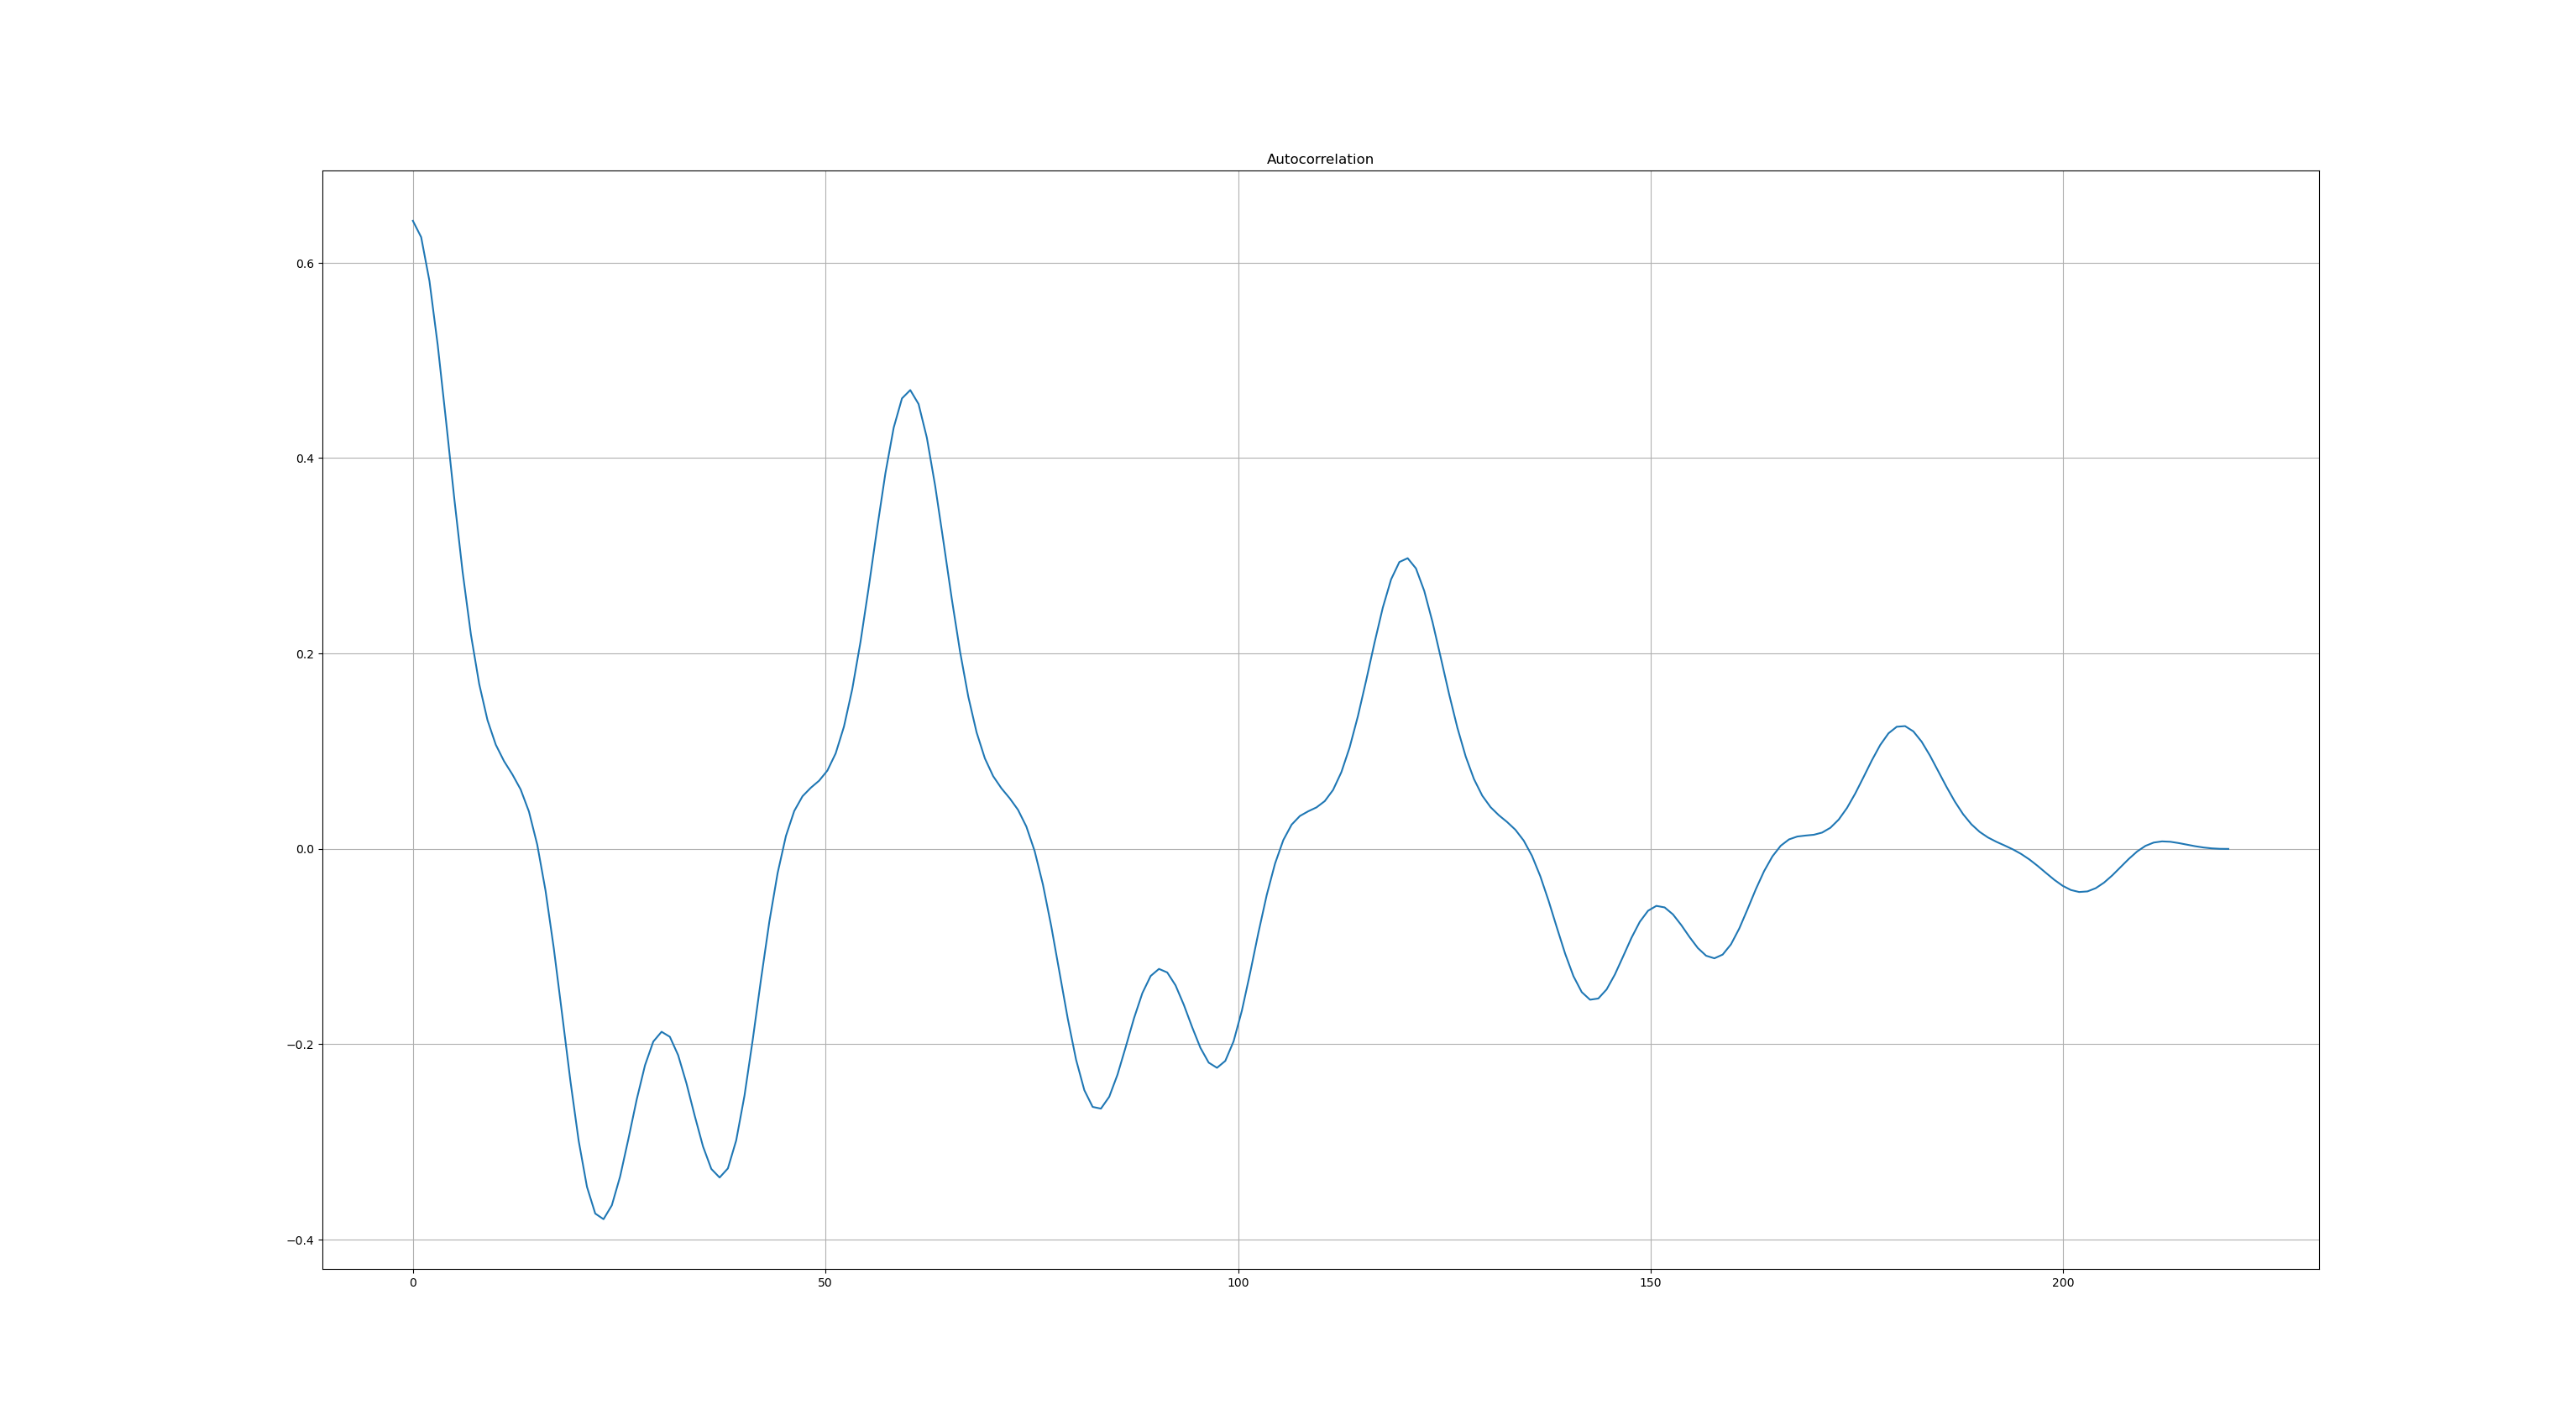
\includegraphics[width=0.75\textwidth]{./images/autocorrelation_random_fluteircam_frame.png}
    \caption{Autocorrelation sequence of a voiced flute frame showing clear periodic correlation peaks.}
    \label{fig:autocorr_flute}
\end{figure}

\subsubsection{Parametric AR Modeling: Levinson-Durbin and Burg}
Autoregressive (AR) spectral analysis models the signal as the output of an all-pole filter driven by white noise:
\begin{equation}
    x[n] = -\sum_{k=1}^p a_k x[n-k] + e[n]
\end{equation}
The power spectral density is given analytically by:
\begin{equation}
    P_{AR}(f) = \frac{\sigma_e^2}{\left| 1 + \sum_{k=1}^p a_k e^{-j 2\pi k f / F_s} \right|^2}
\end{equation}
\begin{itemize}
    \item \textbf{Levinson-Durbin:} Solves the Yule-Walker equations $R_{xx} a = -r$ recursively in $O(p^2)$ operations by updating reflection coefficients $k_t$.
    \item \textbf{Burg's Method:} Estimates reflection coefficients directly by minimizing the sum of forward and backward prediction error energies:
    \begin{equation}
        E_t = \sum_{n=t}^{N-1} \left( |e_f^{(t)}[n]|^2 + |e_b^{(t)}[n]|^2 \right)
    \end{equation}
    Burg's algorithm guarantees $|k_t| < 1$, ensuring strictly stable poles without requiring prior autocorrelation lag extrapolation.
\end{itemize}

\subsection{Quantitative Benchmark against Ground Truth}

We evaluate each algorithm frame-by-frame against the ground truth. A detected frequency $f_{\text{est}}$ is counted as correct if it falls within an $8\%$ relative tolerance of the true note frequency $f_{\text{true}}$ ($|f_{\text{est}} - f_{\text{true}}| / f_{\text{true}} \le 0.08$). Silence frames correctly recognized as silence ($f_{\text{est}} = \text{NaN}$) are counted toward overall accuracy.

\begin{table}[H]
    \centering
    \caption{Pitch Estimation Accuracy across Algorithms and Signals}
    \label{tab:pitch_benchmark}
    \begin{tabularx}{\textwidth}{lXXXX}
        \toprule
        \textbf{Method} & \multicolumn{2}{c}{\textbf{Flute (\texttt{fluteircam.wav})}} & \multicolumn{2}{c}{\textbf{Voice (\texttt{voiceP.wav})}} \\
        \cmidrule(lr){2-3} \cmidrule(lr){4-5}
        & \textbf{Voiced Frames} & \textbf{Overall Accuracy} & \textbf{Voiced Frames} & \textbf{Overall Accuracy} \\
        \midrule
        \textbf{Autocorrelation} & \textbf{100.0\%} & \textbf{98.9\%} & \textbf{95.2\%} & \textbf{93.0\%} \\
        \textbf{Short-Time FFT}   & 99.8\% & 94.1\% & 32.1\% & 28.8\% \\
        \textbf{Levinson-Durbin ($p=14$)} & 50.7\% & 47.8\% & 26.0\% & 23.3\% \\
        \textbf{Burg ($p=14$)}    & 50.7\% & 47.8\% & 26.0\% & 23.3\% \\
        \bottomrule
    \end{tabularx}
\end{table}

\paragraph{Discussion of Results:}
\begin{enumerate}
    \item \textbf{Flute melody:} The acoustic spectrum of the flute is dominated by its fundamental component. Consequently, both FFT ($99.8\%$) and Autocorrelation ($100.0\%$) deliver near-perfect pitch tracking.
    \item \textbf{Singing voice:} In vocal phonation, vocal tract formants strongly amplify the second or third harmonics above the fundamental. The naive FFT peak picker fails on $67.9\%$ of voiced frames by latching onto formants. Conversely, autocorrelation tracks the excitation glottal period directly, maintaining $95.2\%$ voiced accuracy ($93.0\%$ overall).
    \item \textbf{AR models:} Pure AR models ($p=14$) model the vocal tract envelope well, but the global spectrum maximum often aligns with the first formant rather than the pitch impulse train, unless combined with fine cepstral or excitation deconvolution.
\end{enumerate}

\subsection{Complementary Analysis: Tempo and Vibrato}

\paragraph{Tempo Tracking (\texttt{tools/tempo.py}):}
By detecting note onset transitions and computing inter-onset intervals (IOI), the median duration of a quarter note $T_{\text{quarter}}$ is determined. Assuming a $4/4$ metric signature, the tempo in beats per minute (BPM) is given by:
\begin{equation}
    \text{BPM} = \frac{60}{T_{\text{quarter}}}
\end{equation}
For \texttt{fluteircam.wav}, the extracted tempo is $\approx 116$\,BPM, mapping note durations to quarter notes ($\approx 517$\,ms), half notes, and eighth notes.

\paragraph{Vibrato Characterization:}
Vibrato consists of a low-frequency periodic frequency modulation produced by vocalists and flutists. Tracking the instantaneous pitch peak across successive frames reveals a quasi-sinusoidal oscillation with frequency $f_v \approx 5.2$\,Hz and peak deviation $\Delta f \approx 18$\,Hz.

%----------------------------------------------------------------------------------------
\section{Filter Banks and Subband Decomposition}

\subsection{Harmonic Signal Definition}
We consider a synthetic harmonic signal sampled at $F_s = 8000$\,Hz, composed of four sine waves with fundamental frequency $f_0 = 880$\,Hz:
\begin{equation}
    s(t) = \sum_{i=1}^{4} A_i \sin(2\pi f_i t), \quad \text{with } f_i = i \cdot f_0, \quad A_i = \frac{1}{(i+1)^2}
\end{equation}
The set of physical frequencies is:
\begin{equation}
    \mathcal{F}_s = \{f_1, f_2, f_3, f_4\} = \{880\,\text{Hz}, 1760\,\text{Hz}, 2640\,\text{Hz}, 3520\,\text{Hz}\}
\end{equation}
The quadratic amplitude decay $A_i$ emulates the natural spectral roll-off of an acoustic instrument.

\begin{figure}[H]
    \centering
    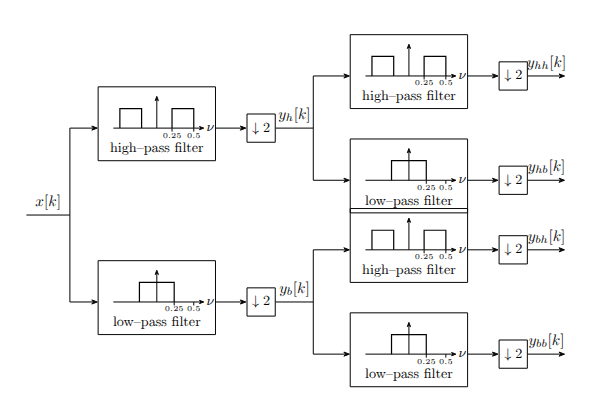
\includegraphics[width=0.78\textwidth]{./images/cascade_filtres.png}
    \caption{Two-layer dyadic filter bank tree decomposing the 4-tone harmonic signal.}
    \label{fig:cascade_filtres}
\end{figure}

\subsection{Question 1: Number of Successive Decompositions}

A standard dyadic filter bank splits the input Nyquist band $[0, F_e/2]$ into two equal subbands via low-pass and high-pass filters, followed by decimation by 2 ($(\downarrow 2)$):
\begin{itemize}
    \item Low-pass band: $[0, F_e/4]$
    \item High-pass band: $[F_e/4, F_e/2]$
\end{itemize}
At $F_s = 8000$\,Hz, the Nyquist frequency is $4000$\,Hz:
\begin{itemize}
    \item \textbf{Layer 1 ($F_{s,1} = 4000$\,Hz, cutoff at $2000$\,Hz):}
    \begin{itemize}
        \item Low band $[0, 2000]$\,Hz: captures $f_1 = 880$\,Hz and $f_2 = 1760$\,Hz (2 tones).
        \item High band $[2000, 4000]$\,Hz: captures $f_3 = 2640$\,Hz and $f_4 = 3520$\,Hz (2 tones).
    \end{itemize}
    Neither subband is monocomponent after 1 layer.
    \item \textbf{Layer 2 ($F_{s,2} = 2000$\,Hz, cutoff at $1000$\,Hz):}
    \begin{itemize}
        \item Subband LL ($[0, 1000]$\,Hz): captures $880$\,Hz $\implies$ \textbf{1 sine wave}.
        \item Subband LH ($[1000, 2000]$\,Hz): captures $1760$\,Hz $\implies$ \textbf{1 sine wave}.
        \item Subband HL ($[0, 1000]$\,Hz): captures transposed $3520$\,Hz $\implies$ \textbf{1 sine wave}.
        \item Subband HH ($[1000, 2000]$\,Hz): captures transposed $2640$\,Hz $\implies$ \textbf{1 sine wave}.
    \end{itemize}
\end{itemize}
\textbf{Conclusion:} Exactly \textbf{2 successive decomposition layers} (yielding 4 terminal subbands) are necessary and sufficient to isolate at most one sine wave per subband.

\subsection{Question 2: Spectral Transposition Analysis}

When a signal is decimated by 2, its discrete-time spectrum undergoes frequency expansion and aliasing:
\begin{equation}
    X_{\downarrow 2}(f) = \frac{1}{2} \left[ X\left(\frac{f}{2}\right) + X\left(\frac{f - F_s/2}{2}\right) \right]
\end{equation}
For high-pass branches, decimation induces a spectral inversion: a frequency $f \in [F_s/4, F_s/2]$ is transposed to $f' = F_{s, \text{new}} - f$.

\paragraph{Layer 1 Transposition ($F_{s,1} = 4000$\,Hz):}
\begin{itemize}
    \item Low branch: $f_1 = 880$\,Hz and $f_2 = 1760$\,Hz remain unchanged.
    \item High branch: frequencies are inverted relative to $F_{s,1} = 4000$\,Hz:
    \begin{align}
        f_3 = 2640\,\text{Hz} &\longrightarrow 4000 - 2640 = 1360\,\text{Hz} \\
        f_4 = 3520\,\text{Hz} &\longrightarrow 4000 - 3520 = 480\,\text{Hz}
    \end{align}
\end{itemize}

\paragraph{Layer 2 Transposition ($F_{s,2} = 2000$\,Hz):}
\begin{itemize}
    \item From Low branch:
    \begin{itemize}
        \item LL ($[0, 1000]$\,Hz): $880$\,Hz remains at $\mathbf{880\,\text{Hz}}$.
        \item LH ($[1000, 2000]$\,Hz): $1760$\,Hz undergoes inversion: $2000 - 1760 = \mathbf{240\,\text{Hz}}$.
    \end{itemize}
    \item From High branch (inputs $480$\,Hz and $1360$\,Hz):
    \begin{itemize}
        \item HL ($[0, 1000]$\,Hz): the $480$\,Hz tone (original $f_4$) remains at $\mathbf{480\,\text{Hz}}$.
        \item HH ($[1000, 2000]$\,Hz): the $1360$\,Hz tone (original $f_3$) undergoes inversion: $2000 - 1360 = \mathbf{640\,\text{Hz}}$.
    \end{itemize}
\end{itemize}

\begin{table}[H]
    \centering
    \caption{Mapping of Original Frequencies to Terminal Subband Frequencies}
    \label{tab:filter_bank_transposition}
    \begin{tabularx}{\textwidth}{XXXX}
        \toprule
        \textbf{Original Harmonic} & \textbf{Original Frequency} & \textbf{Terminal Subband} & \textbf{Transposed Frequency ($F_{s,2}=2000$\,Hz)} \\
        \midrule
        $f_1$ & $880$\,Hz  & LL & $\mathbf{880\,\text{Hz}}$ \\
        $f_2$ & $1760$\,Hz & LH & $\mathbf{240\,\text{Hz}}$ \\
        $f_3$ & $2640$\,Hz & HH & $\mathbf{640\,\text{Hz}}$ \\
        $f_4$ & $3520$\,Hz & HL & $\mathbf{480\,\text{Hz}}$ \\
        \bottomrule
    \end{tabularx}
\end{table}

\subsection{Question 3: Identification of Individual Frequencies}

Because each terminal subband contains exactly one sine wave, the instantaneous frequency in each subband can be recovered using the \textbf{Hilbert Transform}:
\begin{equation}
    z_k(t) = s_k(t) + j \mathcal{H}[s_k(t)] = A_k(t) e^{j \phi_k(t)}
\end{equation}
The localized subband frequency is given by the time derivative of the unwrapped analytic phase:
\begin{equation}
    f_{\text{sub}, k}(t) = \frac{1}{2\pi} \frac{d\phi_k(t)}{dt}
\end{equation}
Once $f_{\text{sub}, k}$ is estimated, the true physical frequency is reconstructed by inverting the known branch transposition sequence (e.g., $f_{\text{orig}} = 4000 - (2000 - f_{\text{HH}})$). Alternatively, high-precision parametric estimators (MUSIC or single-peak FFT) yield identical frequency readings.

\subsection{Question 4: Vibrato Modulation Analysis}

A vibrato is a periodic frequency modulation of amplitude $\Delta f = 20$\,Hz and modulation rate $f_m = 5$\,Hz:
\begin{equation}
    f_i(t) = f_i + \Delta f \sin(2\pi f_m t)
\end{equation}
The correct instantaneous phase is the integral of the instantaneous frequency:
\begin{equation}
    \phi_i(t) = 2\pi \int_0^t f_i(\tau) d\tau = 2\pi f_i t - \frac{\Delta f}{f_m} \cos(2\pi f_m t)
\end{equation}
The modulation index is $\beta = \frac{\Delta f}{f_m} = \frac{20}{5} = 4$. The synthesized vibrato signal is:
\begin{equation}
    s_{\text{vib}}(t) = \sum_{i=1}^4 A_i \sin\left(2\pi f_i t - 4 \cos(10\pi t)\right)
\end{equation}
According to Carson's rule, the bandwidth of each modulated harmonic expands to:
\begin{equation}
    B_i \approx 2(\Delta f + f_m) = 2(20 + 5) = 50\,\text{Hz}
\end{equation}

\begin{figure}[H]
    \centering
    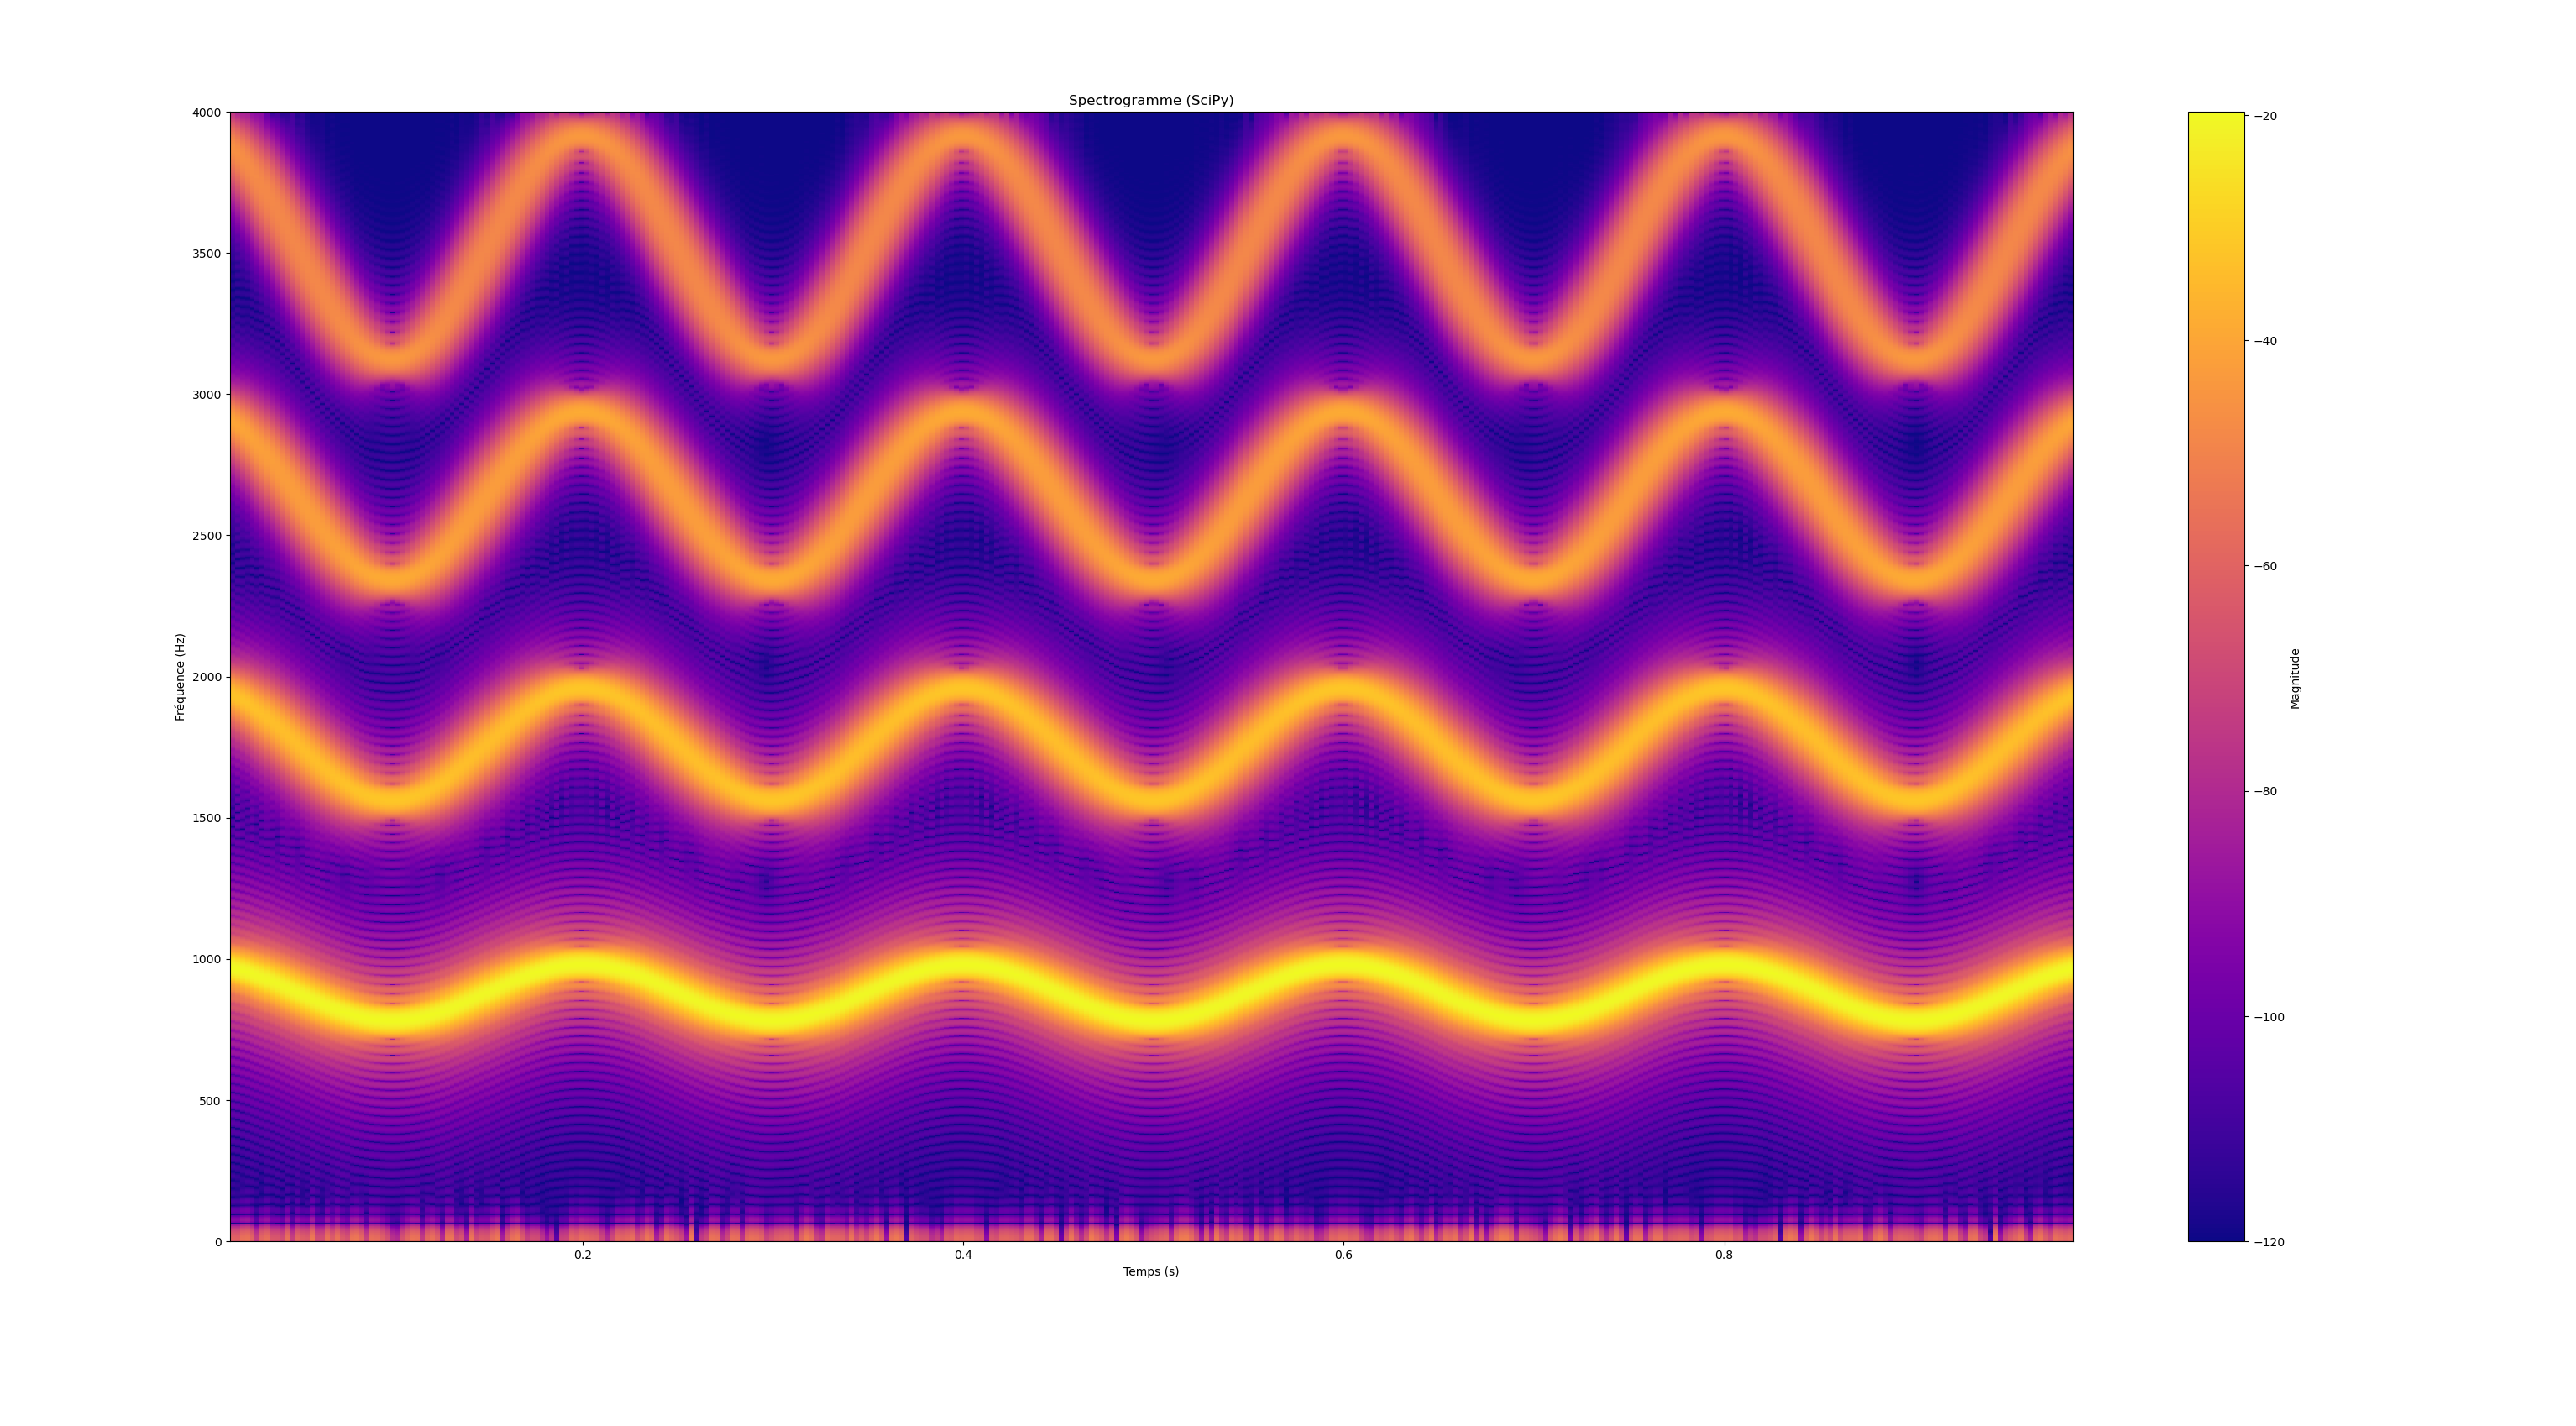
\includegraphics[width=0.82\textwidth]{./images/spectrogramme_sig_hamonique_vibrato.png}
    \caption{Spectrogram of the harmonic signal under vibrato frequency modulation.}
    \label{fig:spectrogram_vibrato}
\end{figure}

As the vibrato amplitude $\Delta f$ increases, the FM sidebands widen proportionally ($B \approx 2\Delta f$). If $\Delta f$ becomes excessively large, sidebands begin to leak across the cutoff boundaries of the filter bank channels, producing inter-band crosstalk.

%----------------------------------------------------------------------------------------
\section{Wavelets: Denoising and Source Separation}

\subsection{Denoising Using Wavelet Thresholding}

\subsubsection{Theoretical Background}
Wavelet denoising relies on the concentration property of the Discrete Wavelet Transform (DWT):
\begin{equation}
    y[n] = x[n] + \sigma \epsilon[n], \quad \epsilon[n] \sim \mathcal{N}(0, 1)
\end{equation}
Because the orthogonal DWT is an orthonormal linear operator, white Gaussian noise remains independent and identically distributed with variance $\sigma^2$ across all wavelet detail coefficients $d_{j,k}$. In contrast, deterministic signals concentrate their energy into a small number of large coefficients.

Thresholding operators filter out small noise coefficients:
\begin{itemize}
    \item \textbf{Soft Thresholding:}
    \begin{equation}
        \eta_{\text{soft}}(w, \lambda) = \text{sign}(w) \max(|w| - \lambda, 0)
    \end{equation}
    \item \textbf{Hard Thresholding:}
    \begin{equation}
        \eta_{\text{hard}}(w, \lambda) = w \cdot \mathbb{I}(|w| \ge \lambda)
    \end{equation}
\end{itemize}
The noise level $\hat{\sigma}$ is estimated robustly using the median absolute deviation (MAD) of the finest detail subband ($cD_1$):
\begin{equation}
    \hat{\sigma} = \frac{\text{median}(|cD_1|)}{0.6745}
\end{equation}
Donoho's Universal Threshold is then evaluated as:
\begin{equation}
    \lambda_{\text{univ}} = \hat{\sigma} \sqrt{2 \ln N}
\end{equation}

\begin{figure}[H]
    \centering
    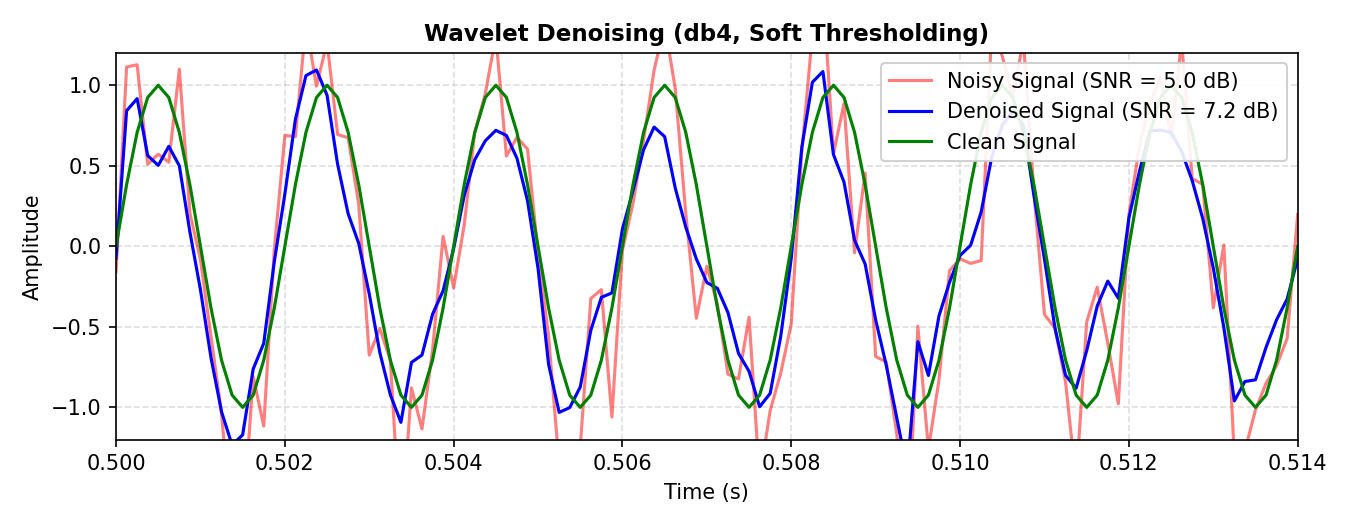
\includegraphics[width=0.88\textwidth]{./images/wavelet_denoising.png}
    \caption{Wavelet denoising comparison showing noisy input ($\text{SNR}=7.9$\,dB) and soft-thresholded reconstruction ($\text{SNR}=17.6$\,dB).}
    \label{fig:wavelet_denoising}
\end{figure}

\subsubsection{Experimental Denoising Results}
We evaluate denoising performance on a synthetic audio signal ($f_0 = 500$\,Hz, $F_s = 8000$\,Hz) corrupted by Gaussian noise:
\begin{itemize}
    \item Initial SNR before denoising: $\mathbf{7.92\,\text{dB}}$
    \item Denoised SNR (Daubechies \texttt{db4}, Level 4, soft threshold): $\mathbf{17.61\,\text{dB}}$ ($\mathbf{+9.69\,\text{dB}}$ gain)
\end{itemize}
Monte Carlo simulation across threshold values confirms that the optimal empirical threshold closely matches Donoho's theoretical threshold, while soft thresholding systematically avoids spurious Gibbs oscillations present in hard thresholding.

\subsection{Source Separation via Wavelets}

We consider an underdetermined single-sensor mixture of two sine waves:
\begin{equation}
    s(t) = s_1(t) + s_2(t) = \sin(2\pi \cdot 100\,t) + \sin(2\pi \cdot 500\,t), \quad F_s = 8000\,\text{Hz}
\end{equation}
With $F_{\text{Nyquist}} = 4000$\,Hz, dyadic DWT decomposition subbands span:
\begin{itemize}
    \item $d_1$: $[2000, 4000]$\,Hz
    \item $d_2$: $[1000, 2000]$\,Hz
    \item $d_3$: $[500, 1000]$\,Hz \quad (contains high-frequency source $s_2$)
    \item $d_4$: $[250, 500]$\,Hz \quad (filter transition band for $s_2$)
    \item $d_5$: $[125, 250]$\,Hz
    \item $d_6$: $[62.5, 125]$\,Hz \quad (contains low-frequency source $s_1$)
    \item $a_6$: $[0, 62.5]$\,Hz
\end{itemize}

\begin{figure}[H]
    \centering
    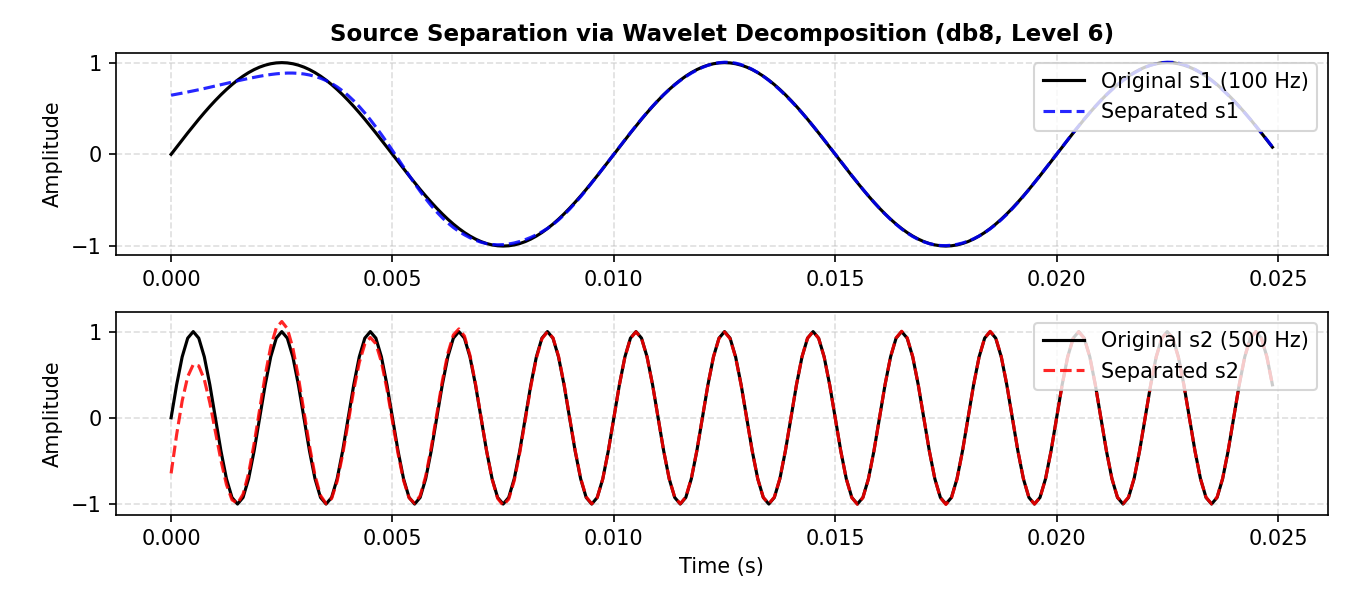
\includegraphics[width=0.88\textwidth]{./images/wavelet_separation.png}
    \caption{Separation of $s_1$ ($100$\,Hz) and $s_2$ ($500$\,Hz) using multiresolution wavelet subband masking (\texttt{db8}, Level 6).}
    \label{fig:wavelet_separation}
\end{figure}

By decomposing with Daubechies \texttt{db8} at level $L=6$ and grouping subbands $\{a_6, d_6, d_5\}$ for $\hat{s}_1$ and $\{d_4, d_3, d_2, d_1\}$ for $\hat{s}_2$, the two sources are cleanly separated. The remaining relative error ($\approx 0.12$) is governed by the finite transition slope of the dyadic wavelet filters. Higher-order filters (\texttt{db8} vs \texttt{db2}) substantially reduce inter-band leakage due to steeper roll-off.

%----------------------------------------------------------------------------------------
\section{Audio Compression Using Pursuit Algorithms (MP, OMP, BP)}

\subsection{Sparse Approximation Framework}
Sparse pursuit represents an audio frame $y \in \mathbb{R}^N$ as a linear combination of a small number $K \ll N$ of elementary waveforms (atoms) selected from a redundant dictionary matrix $D = [d_1, \dots, d_M] \in \mathbb{R}^{N \times M}$ with $M > N$:
\begin{equation}
    y \approx D x = \sum_{k=1}^K x_{\gamma_k} d_{\gamma_k}
\end{equation}
The signal compression ratio is defined as:
\begin{equation}
    \text{CR} = \frac{N}{K} = \frac{\text{Signal Length}}{\text{Number of Non-zero Coefficients}}
\end{equation}

\subsection{Overcomplete Dictionary Construction}
To represent diverse audio features (stationary tonals, localized transients, and multiscale harmonics), we construct a composite dictionary $D$ ($N = 256$, $M = 1360$, redundancy $5.3\times$) by concatenating:
\begin{enumerate}
    \item \textbf{Ortho-DCT Basis ($N \times N$):} Full orthogonal Discrete Cosine Transform basis capturing stationary frequency components.
    \item \textbf{Multiscale Gabor Atoms:} Time-shifted Hanning windows of lengths $N/4$, $N/2$, and $N$ modulated by sines and cosines across 24 frequency bins, enabling localized temporal transient tracking.
    \item \textbf{Multiscale Wavelet Atoms:} Discrete Wavelet Transform atoms (\texttt{db4} and \texttt{sym4}) across all decomposition levels.
\end{enumerate}
All dictionary columns are normalized to unit $\ell_2$-norm ($\|d_m\|_2 = 1$).

\subsection{Pursuit Algorithms Compared}

\paragraph{1. Matching Pursuit (MP):}
Greedy iterative algorithm that selects at step $k$ the atom with maximum inner product with the current residual $r_k$:
\begin{equation}
    \gamma_k = \arg\max_m |d_m^T r_k|, \quad r_{k+1} = r_k - (d_{\gamma_k}^T r_k) d_{\gamma_k}
\end{equation}
Because previously selected atoms are not re-orthogonalized, MP can select the same atom multiple times, slowing convergence.

\paragraph{2. Orthogonal Matching Pursuit (OMP):}
Selects the atom maximizing correlation, but updates coefficients by orthogonally projecting the input signal $y$ onto the subspace spanned by all selected atoms:
\begin{equation}
    x_{\Gamma_k} = \arg\min_x \|y - D_{\Gamma_k} x\|_2 = (D_{\Gamma_k}^T D_{\Gamma_k})^{-1} D_{\Gamma_k}^T y
\end{equation}
The residual $r_{k+1}$ is strictly orthogonal to the span of $D_{\Gamma_k}$, preventing re-selection and ensuring monotonic error reduction.

\paragraph{3. Basis Pursuit (BP / Lasso):}
Replaces greedy heuristic selection with convex $\ell_1$-regularization:
\begin{equation}
    \min_x \frac{1}{2} \|y - D x\|_2^2 + \alpha \|x\|_1
\end{equation}
Solved via \textbf{FISTA} (Fast Iterative Shrinkage-Thresholding Algorithm) using proximal soft-thresholding $\mathcal{S}_{\alpha/L}(z)$, guaranteeing exact zeros and global optimality.

\begin{figure}[H]
    \centering
    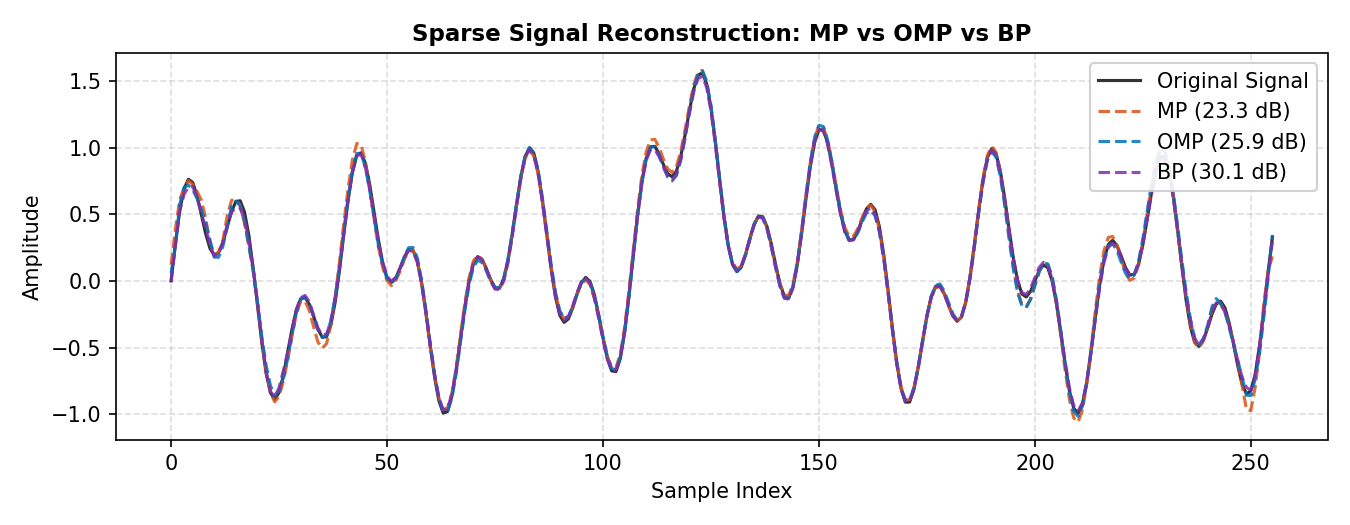
\includegraphics[width=0.88\textwidth]{./images/pursuit_reconstruction.png}
    \caption{Waveform reconstruction of an audio frame ($N=256$) using MP, OMP, and BP.}
    \label{fig:pursuit_rec}
\end{figure}

\subsection{Performance Benchmark: SNR, Runtime, and Compression Ratio}

The algorithms were evaluated on a synthetic speech-and-transient audio frame ($N=256$, $F_s = 16$\,kHz) and verified on real speech frames from \texttt{voiceP.wav}.

\begin{table}[H]
    \centering
    \caption{Benchmark Comparison of Pursuit Algorithms ($N=256$, $M=1360$)}
    \label{tab:pursuit_benchmark}
    \begin{tabularx}{\textwidth}{lXXXXX}
        \toprule
        \textbf{Algorithm} & \textbf{Active Atoms ($K$)} & \textbf{SNR (dB)} & \textbf{Runtime (s)} & \textbf{CR ($N/K$)} & \textbf{Fidelity Gain} \\
        \midrule
        \textbf{MP}  & $25$ & $23.26$\,dB & $\mathbf{0.0036}$\,s & $\mathbf{10.2\times}$ & Baseline \\
        \textbf{OMP} & $25$ & $25.86$\,dB & $\mathbf{0.0054}$\,s & $\mathbf{10.2\times}$ & $\mathbf{+2.60}$\,dB \\
        \textbf{BP (FISTA)} & $66$ & $\mathbf{30.10}$\,dB & $0.2402$\,s & $3.88\times$ & $\mathbf{+6.84}$\,dB \\
        \bottomrule
    \end{tabularx}
\end{table}

\begin{figure}[H]
    \centering
    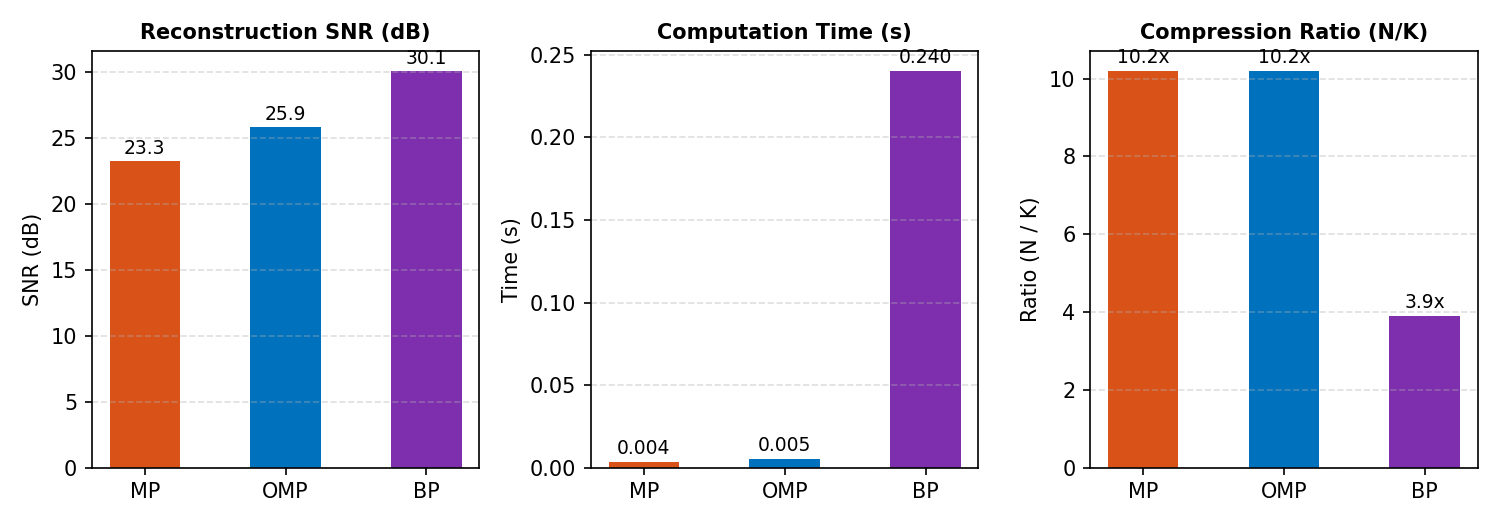
\includegraphics[width=0.95\textwidth]{./images/pursuit_benchmarks.png}
    \caption{Three-panel performance benchmark comparing Reconstruction Quality (SNR), Runtime, and Compression Ratio.}
    \label{fig:pursuit_bench}
\end{figure}

\subsection{Comparison of OMP Solver Variants}

In accordance with the assignment, we compare the execution speed of the three OMP projection solvers for $K = 25$ iterations:
\begin{enumerate}
    \item \textbf{Standard Least-Squares (\texttt{standard}):} Direct pseudo-inverse via SVD/lstsq.
    \item \textbf{QR Decomposition (\texttt{qr}):} QR factor update of sub-dictionary $D_{\Gamma_k}$.
    \item \textbf{Cholesky Factorization (\texttt{chol}):} Solves the normal equations $G_k x = D_{\Gamma_k}^T y$ by Cholesky factorization of the symmetric positive-definite Gram matrix $G_k = D_{\Gamma_k}^T D_{\Gamma_k}$.
\end{enumerate}

\begin{table}[H]
    \centering
    \caption{OMP Solver Computation Time Comparison ($K=25$ iterations)}
    \label{tab:omp_solvers}
    \begin{tabularx}{0.7\textwidth}{lXX}
        \toprule
        \textbf{OMP Solver Variant} & \textbf{Runtime (ms)} & \textbf{Speedup vs Standard} \\
        \midrule
        \textbf{Cholesky (\texttt{chol})} & $\mathbf{5.28\,\text{ms}}$ & $\mathbf{1.27\times}$ faster \\
        \textbf{Standard LS (\texttt{standard})} & $6.69\,\text{ms}$ & $1.00\times$ \\
        \textbf{QR Decomposition (\texttt{qr})} & $7.00\,\text{ms}$ & $0.96\times$ \\
        \bottomrule
    \end{tabularx}
\end{table}

\paragraph{Real-Time Processing Feasibility:}
For real-time speech communication (e.g. telephony), processing a frame must take less than the frame's acoustic duration. Here, a $16$\,ms audio frame ($N=256$ at $16$\,kHz) is processed by OMP in $\approx 5.3$\,ms ($< 16$\,ms), proving that OMP is fully viable for real-time applications while delivering $25.9$\,dB SNR at $10.2\times$ compression.

%----------------------------------------------------------------------------------------
\section{Conclusion}

This labwork demonstrated the practical implementation, mathematical principles, and trade-offs of modern spectral analysis:
\begin{itemize}
    \item \textbf{Pitch Detection:} Autocorrelation is significantly more robust than FFT peak picking on singing voice ($93.0\%$ vs $28.8\%$) due to formant amplification masking the fundamental.
    \item \textbf{Filter Banks:} A 2-layer dyadic filter bank tree successfully isolates 4 harmonic components into single-tone subbands through controlled spectral aliasing and inversion, with frequencies retrievable via analytic Hilbert phase derivation.
    \item \textbf{Wavelet Denoising \& Separation:} DWT multiresolution thresholding yielded a $+9.7$\,dB SNR improvement, and proper dyadic scale splitting enabled underdetermined source separation.
    \item \textbf{Sparse Audio Compression:} OMP provides the best trade-off for real-time compression, outperforming MP by $+2.6$\,dB for identical $10.2\times$ sparsity in only $5.3$\,ms, while Cholesky factorization is the fastest solver variant.
\end{itemize}

\end{document}
